\chapter{System Design and Architecture}

\section{Introduction}

This chapter presents a technical framework and architecture for implementing an embedded self-documenting DSL that is written in Scheme.  In addition to the DSL, this chapter will also different ontologies that will be used to model data.  The proposed DSL provides human-friendly syntax that allows a user to select tables from a SQL database, translate them into RDF, and save the output in a specified file, all while generating a markdown file that has documentation about that given dump.  Given the DSL's foundation in Scheme, end users are also able to leverage Scheme's capabilities within the DSL's framework, thereby enhancing its extensibility.

\section{Design Process}

\subsection{Design Goals}

In contrast to general-purpose languages (GPLs), DSLs present certain benefits, as highlighted by \citet{freudenthal2010domain} and \citet{spinellis2001notable}:

\begin{enumerate}
\item \textit{Explicit Representation of Domain Knowledge:} DSLs allow domain-specific functionality to be expressed in a tangible, human-readable format at a high level of abstraction.  This clarity makes software artifacts more accessible to developers, thereby simplifying the processes of development, testing and modification.
\item \textit{Active Engagement of Domain Experts:} Programs crafted in DSL often adopt a style that aligns with the conventional formats used by domain experts.  This facilitates their participation in the software's lifecycle and promotes collaboration with developers. In some cases, domain experts might directly specify, implement, verify or validate certain artifacts.
\end{enumerate}

In lieu of the aforementioned advantages of a DSL, the system architecture should accomplish the following:

\begin{enumerate}
\item The architecture must be \textit{database agnostic.}  Given that users will be employing this DSL with their unique databases, it is essential for the DSL to be flexible enough to support constructs that allows them to work with their unique database.
\item The architecture should empower users to model, in the context of some defined ontology, the mapping of the results derived from their SQL queries into RDF.
\item The DSL should provide a means of self-documenting itself while transforming data from SQL to RDF.
\end{enumerate}

\subsection{Architecture}
TODO
%% To achieve the design goals outlined above, the layered architectural pattern \citep{richards2015software} is used.  The DSL is organized into four primary layers:

%% \begin{enumerate}
%% \item The first layer encompasses the Input-Output operations related to a file.
%% \item The second layer embodies the processes of adding an RDF prefix and defining a dump that works on a single table.
%% \item The third layer portrays the semantic elements needed to define a dump.
%% \item The final layer illustrates the potential operations that can be nested when defining an RDF triple.
%% \end{enumerate}
    
%% The structure of these layers is visualized in Figure \ref{fig:layered-arch}.

%% \begin{figure}[H]
%%   \centering
%%   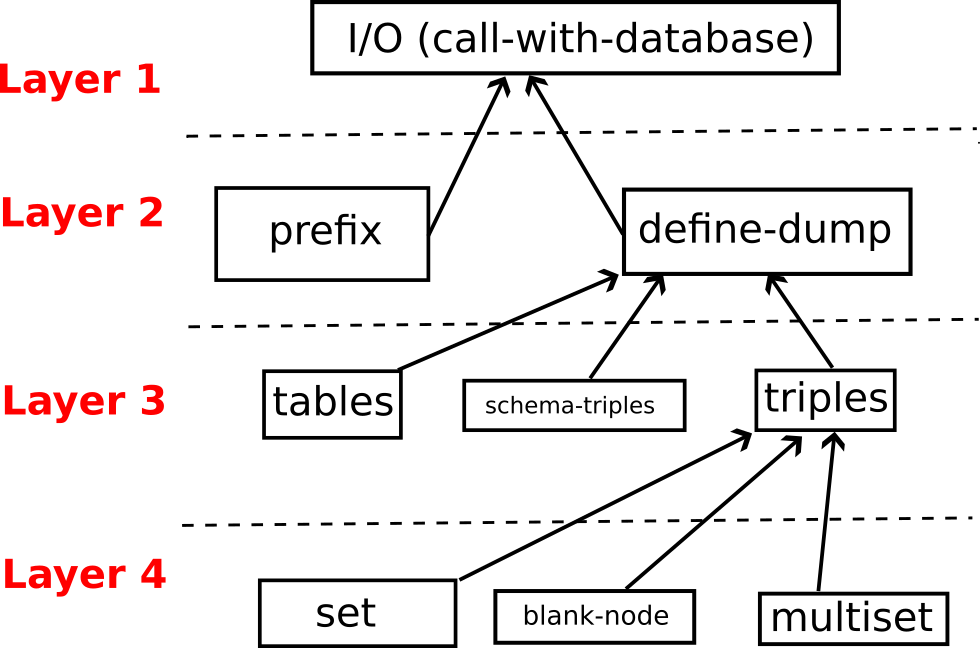
\includegraphics[width=12cm]{archLayers}
%%   \caption{\textit{Architecture layers}}
%%   \label{fig:layered-arch}
%%   \centering
%% \end{figure}

%% \subsubsection{Layer 1}

%% This layer contains the I/O operation: \textit{call-with-database}.  This allows a database connection that can be passed down to functions defined in the layers below it.

%% \subsubsection{Layer 2}

%% ``prefix'' allows the user to define a given RDF prefix, and ``define-dump'' allows them to model a given table that will be dumped.  ``define-dump'' depends on elements of Layer 3 to operate.

%% \subsubsection{Layer 3}
%% This layer is where most of the modelling happens.  All elements in this layer are composed together to form ``define-dump'' as follows:

%% The \texttt{tables} clause specifies the database tables to be joined to construct the view to be parsed.  \texttt{TABLE} can be in the form \texttt{TABLE-NAME} or of the form \texttt{JOIN-OPERATOR TABLE-NAME RAW-CONDITION}.  \texttt{TABLE-NAME} is the name of the target table.  The \texttt{JOIN-OPERATOR} can be either a join, left-join or an inner-join.  \texttt{RAW-CONDITION} is the join condition as a raw string, for example \texttt{``USING (SpeciesId)''}.  \texttt{RAW-FORMS} are expressions that should evaluate to strings which will be appended to the SQL query during macro-expansion.

%% The \texttt{schema-triples} clause identifies the list of triples written once when the dump begins.

%% The triples clause specifies the triples to be dumped once for each row in the view.  All triples have a common \texttt{SUBJECT}. The \texttt{(verb predicate object)} clauses are described below:

%% \begin{itemize}
%% \item \texttt{VERB} must either be a set or multiset. For the set \texttt{VERB}, a single triple \texttt{(SUBJECT PREDICATE OBJECT-VALUE)} is written where \texttt{OBJECT-VALUE} is the result of evaluating \texttt{OBJECT}. For the multiset \texttt{VERB}, \texttt{OBJECT} must evaluate to a list, and a triple \texttt{(SUBJECT PREDICATE OBJECT-VALUE-ELEMENT)} is created for each element \texttt{OBJECT-VALUE-ELEMENT} of that list.
%% \item The \texttt{SUBJECT} and \texttt{OBJECT} expressions in the triples clause must reference database fields using a \texttt{(field TABLE COLUMN)} clause where \texttt{TABLE} and \texttt{COLUMN} refer to the table and column of the field being referenced. Database fields can also be referenced using \texttt{(field TABLE COLUMN ALIAS)} where \texttt{ALIAS} is an alias for that column in the SQL query.
%% \end{itemize}

%% \subsubsection{Layer 4}

%% The ``triples'' from the previous layer can have a:

%% \begin{enumerate}
%% \item \textit{set:} represents a single element.
%% \item \textit{multiset:} represents multiple elements.
%% \item \textit {blank-node:} represents the concept of a blank-node which is a native RDF construct.
%% \end{enumerate}

